\documentclass[12pt,a4paper]{report}

\usepackage[utf8x]{inputenc}
\usepackage[francais]{babel}
\usepackage[T1]{fontenc}
\usepackage{amsmath}
\usepackage{amsfonts}
\usepackage{amssymb}
\usepackage[square,sort,comma,numbers]{natbib}
\usepackage[colorlinks=true,linkcolor=blue]{hyperref}
\usepackage{glossaries}
\usepackage[usenames,dvipsnames]{xcolor}
\usepackage{setspace}
\usepackage{graphicx}
\usepackage{float}
\usepackage[skip=2pt,font=scriptsize]{caption}
\usepackage{listings}


\author{Nicolas JEANNE}
\title{Rapport de stage de M2}
\date{11 mars 2015}

% Mise en page des citations
\bibliographystyle{abbrvnat}
\setcitestyle{authoryear,open={(},close={)},aysep={},citesep={;}}


% formattage des entrées du glossaire
\renewcommand*{\glstextformat}[1]{\textcolor{Black}{#1}}
% création des acronymes du glossaire
\newacronym{rep}{REP}{Repeated Extragenic Palindrome}
\newacronym{bime}{BIME}{Bacterial Interspesed Mosaic Element}
\newacronym{sra}{SRA}{Sequence Read Archive}
\newacronym{ngs}{NGS}{Next Generation Sequencing}
\newacronym{sam}{SAM}{\href{http://samtools.github.io/hts-specs/SAMv1.pdf}{Sequence Alignment Map format}}
\newacronym{bam}{BAM}{Binary Alignment Map format}
% création des entrées du glossaire
\newglossaryentry{PE}{name={Paired-end},description={Technique de séquençage haut débit consistant à réaliser les amplifications d'un fragment d'ADN en marquant l'extrémité 5' par un tag \no1 et l'extrémité 3' par un tag \no2. La distance entre les 2 tags est connue et fixe (négative ou jusqu'à 500 pb). Ceci permet lors de l'assemblage, de séquences de 35 pb par exemple, d'associer le read 1 et le read 2 grâce à la distance séparant les 2 et cela même si la séquence intermédiaire est inconnue. Si la distance est négative, il est possible d'obtenir des reads chevauchants de longueur plus importante que les 35 pb}}
\newglossaryentry{reads}{name={reads},description={Séquence nucléotidique issue d'un séquençage NGS}}
\makeglossaries

% Encadrement des figures
\floatstyle{boxed}
\restylefloat{figure}

% Configuration des liens
\hypersetup{
  colorlinks,
  citecolor=Violet,
  linkcolor=Black,
  urlcolor=Blue}

% Configuration des parties de code pour accepter les caractères spéciaux
\lstset{basicstyle=\ttfamily}

\begin{document}

\maketitle

\begin{onehalfspace}
\chapter*{Introduction}
En 1982, la découverte par Higgins et al. de nouveaux éléments génétiques communs dans les régions intercistroniques des opérons de Escherichia coli et Salmonella typhimurium a constitué le premier pas de la recherche sur les \gls{rep} \citep{Higgins1982}. En 1991, Gilson et al. ont mis en évidence l'organisation en clusters de ces REP \citep{Gilson1991}, ces clusters ont été caractérisés comme \gls{bime}. Chez E. coli en 1994, Bachelier et al. ont réussi à catégoriser les REP constituant les BIME en 2 types Y et Z, constituants 3 motifs Y, Z\textsuperscript{1}, Z\textsuperscript{2}  \citep{Bachellier1994}.
 
Les REP constituent une part non négligeable du génome bactérien, chez E. coli K12 ou S. typhimurium elles représentent environ 1\% de celui-ci \citep{Gilson1991}. Nous les retrouvons chez de nombreux règnes bactériens, notamment chez les pathogènes humains tels que \textit{Escherichia coli, Salmonella enterica, Neisseria meningitidis, Mycobacterium tuberculosis et Pseudomonas aeruginosa} mais également chez des pathogènes des plantes comme \textit{Agrobacterium tumefaciens} ou chez des bactéries ubiquitaires, \textit{Deinococcus radiodurans} ou \textit{Pseudomonas putida} par exemple. Les travaux précédents de l'équipe ont permis l'annotation des REP au sein du génome d'E. coli et de mettre en évidence le lien existant entre la prolifération des REP et le gène $tnpA_{REP}$ \citep{Weyder2013,Bosc2014}, ainsi que la reconstruction des états ancêtres des REP \citep{Bosc2014}.  \textcolor{red}{Le rôle exact des REP n'est pas clairement défini, des hypothèses sont avancées sur leur implication dans la régulation de l'expression des gènes, que ce soit en tant que terminateur ou comme site de reconnaissance des enzymes impliquées dans les mécanismes de la transcription.}

\section*{Caractéristiques des REP et organisations en BIME}
La taille des REP varie de 20 à 40 nucléotides, la classification Y, Z\textsuperscript{1}, Z\textsuperscript{2} est basée à la fois sur la taille de la séquence consensus de la REP ainsi que sur sa structure secondaire. Par convention, une REP en orientation inversée est nommée iREP (inversed REP) \citep{Ton-Hoang2012}. Un tétra-nucléotide caractéristique de séquence GTAC est présent à l'extrémité 5' des REP, sa séquence complémentaire est CTAC en 3' pour les iREP. Les différentes classes de REP partagent des nucléotides conservés (\autoref{fig:fig1}A). La structure secondaire des REP est caractérisée par sa forme en tige-boucle, le caractère palindromique permet la formation de la tige malgré un mésappariement situé dans la partie centrale de celle-ci (\autoref{fig:fig1}B). Pour le génome d'E. coli K-12, 93 REP ont été répertoriées comme étant uniques sur les 605 annotées par le laboratoire, les autres sont organisées par paires sous forme de BIME. Une classification a été adoptée comportant 3 entrées, les BIME-1 composées de REP Z\textsuperscript{1} et Y apparaissant en paires uniques et dans lesquelles la REP et l'iREP sont séparées par un linker de séquence longue (L) pouvant lier l'IHF (Integration Host Factor). Les BIME-2 constituées de Z\textsuperscript{2} et de Y, apparaissant en copies multiples de cette paire dont la REP et l'iREP sont séparées par un linker court (S) et une des trois séquences flanquantes (s, l ou r). La troisième catégorie est constituée des BIME dites atypiques qui sont des chimères de BIME-1 et BIME-2, comportant différentes combinaisons de Y, Z\textsuperscript{1}, Z\textsuperscript{2}, S, L, s, l et r. Tout comme les BIME-2, nous les retrouvons sous forme de copies multiples (\autoref{fig:fig1}C).

\begin{figure}[ht]
\centerline{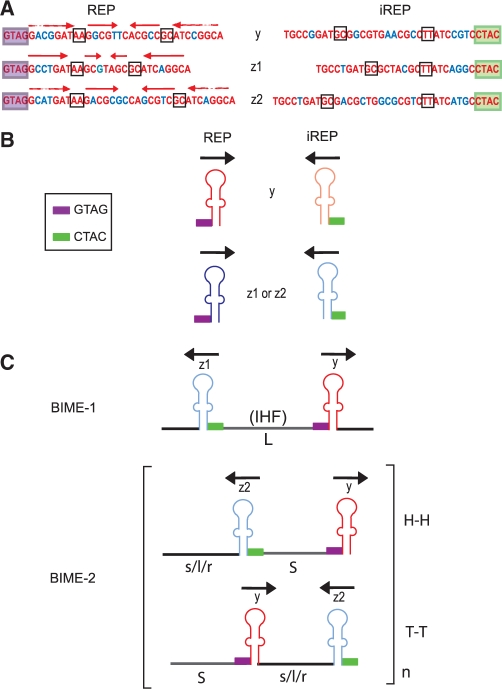
\includegraphics[scale=1.8]{figures/fig1.jpg}}
\caption{\textbf{REP et BIME chez Escherichia coli. (A)} Séquences consensus Y, Z\textsuperscript{1} et Z\textsuperscript{2} des REP. Le tétra-nucléotide conservé GTAC est encadré en violet, le complémentaire conservé CTAC est encadré en vert, les flèches rouges situent les zones d'appariement de la tige et les positions encadrées en noir sont les zones de mésappariement. Les positions conservées parmi les classes de REP sont en rouge, les positions variables en bleu. \textbf{(B)} Structure secondaire des REP. Les rectangles violets et verts représentent respectivement les tétra-nucléotides conservés GTAC pour les REP et CTAC pour les iREP. Les flèches noires indiquent l'orientation des REP. \textbf{(C)} Structures des BIME-1 et BIME-2. Les BIME-1 sont composées de REP et de iREP Y et Z\textsuperscript{1} séparées par un linker de séquence longue (L), les BIME-2 sont composées de Y et Z\textsuperscript{2}, de linker courts (S) et de séquences séparatrices s, l ou r. H-H et T-T dénotent respectivement une organisation tête à tête et queue à queue des REP. \citep{Ton-Hoang2012}.}\label{fig:fig1} 
\end{figure}

\section*{Propriétés associées aux REP}
La littérature décrit de nombreuses fonctions associées aux REP, mais certaines d'entre elles restent encore peu étudiées. Les REP ont été décrite comme jouant un rôle dans les événements de recombinaisons homologues \citep{Kofoid2003}. Les BIME ont été décrites comme des sites privilégiés pour l'insertion de séquences d'ADN mobiles comme certaines familles d'IS (Insertion Sequence) \citep{Bachellier1997,Clement1999,Choi2003,Tobes2005}. Lorsqu'elles sont transcrites, les REP joueraient un rôle dans la stabilisation de l'ARNm grâce à leur structure en tige-boucle \citep{Newbury1987,Espeli2001,Khemici2004,Aguena2009}, la terminaison de la transcription \citep{Gilson1986} et le contrôle de la traduction \citep{Stern1988}. Au niveau de l'ADN, les REP sont capables de lier plusieurs facteurs protéiques tels que l'ADN Gyrase \citep{Espeli1997} et l'ADN polymérase \citep{Gilson1990}. Plus spécifiquement, la BIME-1 peut lier l'IHF sur son linker \citep{Boccard1993} qui peut être notamment responsable de l'initiation de la transcription et d’événements de recombinaisons sites spécifiques \citep{Goosen1995}.

\section*{Transcription chez E. coli}

\subsection*{Stabilité des ARN}

\chapter*{Matériel \& Méthodes}

\section*{Données}
Les données que nous avons exploité sont issues des expériences d'évolution adaptatives en laboratoire visant à découvrir l'émergence de mutations clés permettant la croissance rapide d'E. coli K-12 MG1655 sur un medium pauvre en glucose \citep{Lacroix2014}. Ces données ont été choisies car elles proviennent d'expériences de RNA-Seq comportant un nombre non négligeable de réplicats (9) pour la condition de croissance en milieu pauvre en glucose (ALE) et 2 réplicats pour le Wild Type (WT) . Il s'agit de données \gls{ngs} publiques, accessibles sur le base de données \href{http://www.ncbi.nlm.nih.gov/geo/query/acc.cgi?acc=GSE61327}{GEO} (Gene Expression Omnibus) du NCBI au format \gls{sra}, séquencées sur Illumina MiSeq à partir d'ARN total extrait des cultures d'E. coli et rétro-transcrit en cDNA. La librairie a été conçue en \gls{PE} et brin spécifique. Grâce au \href{http://www.ncbi.nlm.nih.gov/books/NBK158900/#SRA_download.how_do_i_use_the_sra_toolki}{SRA toolkit} et à la commande \texttt{fastq-dump}, elles sont décompressées au format \texttt{fastq}. Un contrôle de qualité a été effectué afin d'inspecter les séquences grâce au logiciel \texttt{fastqc}. Les 2 WT et 8 ALE ont été validés puisque disposant d'une qualité de séquence par base supérieure à 30 pour des \gls{reads} de 62 pb. Seul le fichier \texttt{SRR1573441.fastq} a été rejeté car la longueur des reads allait de 35 à 502 pb avec des scores de qualités très variables.

\section*{Alignement des reads}
Les reads ont été alignés grâce au logiciel \href{http://bio-bwa.sourceforge.net/}{BWA} sur le génome d'E. coli \href{http://www.ncbi.nlm.nih.gov/nuccore/NC_000913.2}{NC\_000913.2} qui est le génome utilisé pour annoter les REP au laboratoire.  Le logiciel BWA propose 3 algorithmes distincts, BWA-backtrack, BWA-SW et BWA-MEM. Pour chacun de ces alignements, il est nécessaire de disposer d'une séquence de référence indexée, obtenue par la commande \texttt{bwa index NC\_000913.2.fasta}. 
L'algorithme que nous avons sélectionné est le MEM (Maximal Exact Matches) car il s'agit du plus récemment développé. Il reprend les mêmes principes que BWA-SW (utilisation de la programmation dynamique pour trouver les seeds en autorisant les mismatchs et les gaps. Il n'étend les alignements des seeds que lorsque ceux-ci ont peu d'occurrences sur le génome de référence, cela permet de diminuer le temps d'alignement en éliminant les extensions des séquences très répétées) mais en utilisant le seeding avec des maximal exact matches, puis il réalise l'extension avec les autorisations de mismatchs et de gaps.
\lstset{language=sh}  
\begin{lstlisting}[frame=single]
bwa mem ref.fasta file.fastq > aln.sam
\end{lstlisting}
Le fichier d'alignement généré est au format \texttt{\gls{sam}}, afin de poursuivre l'analyse il doit être convertit au format binaire \texttt{\gls{bam}}. Cette opération a aussi le mérite de compresser l'information et de gagner de l'espace de stockage. Les séquences vont ensuite être triées par position génomique, puis les duplicats de PCR vont être éliminés.
Si nous déroulons les étapes d'un séquençage haut dédit, nous obtenons :
\begin{enumerate}
\item Fractionnement de l'ADN de l'échantillon.
\item Ligation des adaptateurs aux 2 extrémités des fragments.
\item amplification par PCR des fragments avec les adaptateurs.
\item Création d'une émulsion huile-eau avec les microbilles et les molécules d'ADN (technologies
Roche ou Ion Torrent) ou expansion des molécules d'ADN sur une flowcell (technologie
Illumina). Le but étant d'atteindre exactement une molécule par bille ou par parcelle sur la
flowcell.
\item Amplification du signal par PCR des séquences spécifiques à chaque bille ou parcelle.
\item Séquençage par la technique propre à chaque technologie, pyroséquençage pour Roche,
détection d'ions semi-conducteurs pour Ion Torrent ou par terminateurs de chaîne réversible
pour Illumina.
\end{enumerate}

Les duplicats de PCR sont générés à la 3\ieme{} étape lors de l'amplification, nous cherchons à augmenter le
signal de chaque segment de l'ADN original, mais il arrive que 2 copies de la même portion d'ADN
aille dans 2 billes ou parcelles différentes, c'est ce que l'on appelle les duplicats de PCR. Ces duplicats
amènent un biais lors du séquençage.

Finalement, le fichier BAM trié sans duplicats doit être indexé pour être visualisable sur un Genome Browser.

Les outils utilisés sont compris dans la suite des \href{http://samtools.sourceforge.net/samtools.shtml}{samtools}.
\lstset{language=sh}  
\begin{lstlisting}[frame=single]
# Conversion du SAM en BAM
samtools view -Sb aln.sam > aln.bam

# Tri en fonction des positions genomiques
samtools sort aln.bam aln_sorted

# Elimination des duplicats de PCR
samtools rmdup -s aln_sorted.bam aln_sorted_noDup.bam

# Indexation du fichier d'alignement
samtools index aln_sorted_noDup.bam
\end{lstlisting}

\textcolor{red}{parler du fait que nous ne recherchons pas une différence d'expression entre 2 conditions}

\end{onehalfspace}


 
% affichage du glossaire
\printglossary[type=\acronymtype ,title=Glossaire]


%\bibliographystyle{unsrtnat}
\bibliography{biblio_rapport}




\end{document}